\documentclass{article}
\setcounter{secnumdepth}{0}
%[a4paper, 11pt]
\usepackage{comment} % enables the use of multi-line comments (\ifx \fi) 
\usepackage{fullpage} % changes the margin

\usepackage{graphicx}
%\usepackage{lscape}
%\usepackage{rotating}
\usepackage{pdflscape}
\usepackage{wrapfig}
\usepackage{gensymb}

\renewcommand{\labelenumii}{\theenumii}
\renewcommand{\theenumii}{\theenumi.\arabic{enumii}.}

\usepackage{enumitem}
\usepackage{subcaption}

\newcommand{\CMwidth}{-1.7cm}
\newcommand{\CMheight}{2.7cm}

\usepackage{hyperref}

\setcounter{secnumdepth}{5}% Include \subsubsection in ToC

\def\changemargin#1#2{\list{}{\rightmargin#2\leftmargin#1}\item[]}
\let\endchangemargin=\endlist 

\begin{document}
%Header-Make sure you update this information!!!!
%\noindent
%\large\textbf{Post/Pre-Lab X Report} \hfill \textbf{FirstName LastName} \\
%\normalsize ECE 100-003 \hfill Teammates: Student1, Student2 \\
%Prof. Oruklu \hfill Lab Date: XX/XX/XX \\
%TA: Adam Sumner \hfill Due Date: XX/XX/XX

\title{Interim Report: Hybrid Methods for Finite Element Meshing}
\author{Jack Bradbrook (psyjb4)}
\date{November 30, 2016}
\maketitle

\tableofcontents

\newpage

\section{Introduction}

The overall aim of this project is to perform the task of refining a Finite Element Mesh (FEM) using a stress based method as is typical of FEM refinement in conjunction with an approach that uses techniques from Artificial Intelligence and Machine Learning. \\

\noindent
Finite Element Analysis (FEA) is a method widely used across different engineering domains to simulate structures under certain conditions. The method works by taking a geometry defined in continuous terms, discretiseing it into a mesh system before calculating the property values for each of the discrete elements. This allows engineers to observe the effect the conditions have on the entire structure, see figure 1. \\ 

\noindent
Success of the project will be determined by implementation of a system that is able to combine the two approaches described above in order to refine a mesh to of a quality comparable to that of a successful stress based method.


\section{Motivation and Background}

Over the past forty years FEA has emerged as a prominent technology for simulating complex real world engineering problems \cite{cite0, DolsakPaper94}. FEA works by solving a system of differential equations with each equation representing a single element in the mesh. By doing this FEA is able to generate highly accurate approximations for the properties of complex physical systems \cite{DolsakPaper94} \cite{IntroductionToFE}. The method can also be highly computationally expensive with the complexity typically increasing exponentially with the model size \cite{DolsakPaper94}. Analysis therefore proves to be highly time consuming and costly for individuals and organisations to conduct \cite{ConsultRuleIntelltSystemFE}. \cite{cite03}\\

\noindent
An important consideration when conducting FEA is the trade-off of a models accuracy against the time in which it can be solved. A major variable determining this trade-off is the models mesh structure which discretizes the problem so that simulation can be run on it. A mesh that is finer is more computationally expensive but also produces results of greater accuracy. It is therefore desirable to generate a mesh which is fine where accuracy is most needed but coarse where it isn't \cite{cite04}. FE meshes are constructed out of nodes (points which are intersections of edges) and elements, either a polygon or a polyhedron between the nodes. Nodes and elements are important concepts as they provide the theoretical framework for reasoning about the other properties of a mesh and hence the overall quality of the model \cite{IntroductionToFE}.\\

\noindent
In every type of analysis that the FE method is used for (thermal, structural, fluid flow, electrical) there is a specific differential equation associated with each of the elements. In order to achieve overall convergence of the model the equations must be solved simultaneously to achieve a value for every discrete element \cite{IntroductionToFE}. For this dissertation project attention will be given specifically to the problem of FEA meshing in the context of static structural analysis where the value calculated across each element is its stress. It makes sense to work on hybrid mesh refinement in the context of static structural analysis as it is perhaps the most common engineering application of the method and as such has the largest body of research that is relevant \cite{DolsakPaper94}\cite{IntroductionToFE}.\\

\noindent
For engineers the value obtained through computing the stresses under a particular set of conditions is feedback on the quality of their design. Ideally the results from an analysis will provide a good understanding of where the design is weak and how concentrated this weakness is. This information is used to either help verify the designs' quality or alternatively inform changes to its geometry or material properties so as to reduce stress on subsequent analysis \cite{cite06}.\\

\noindent
To understand the gradient of stress within a part of the model the mesh needs to be designed carefully. As each element can only display values calculated from its edge nodes a smooth gradient requires a higher concentration of elements in areas under higher stress. A high quality mesh is therefore considered to have a higher concentration of elements in areas of predicted high stress while retaining lower concentration elsewhere, thereby revealing weaknesses in the design while minimising the models runtime.\\

\noindent
Traditionally the automated mesh refinement process consists of computing stresses for a model with an initial coarse mesh and low computation cost, once rough stresses have been computed the elements in areas of higher stress can be divided recursively into additional elements in order to achieve smoother gradients on further executions \cite{cite03}. Figure 1 shows a mesh which has been refined in an area of higher stress thus providing a clearer indication of a components weakness. \\ 

\noindent
Unfortunately for many large models this method for refining a mesh is still excessively costly \cite{DolsakPaper91}. It therefore seems worth investigating use of alternative approaches posed by the field of computer science and artificial intelligence that could support the traditional high stress meshing approach. 

\begin{figure}
  \centerline{\includegraphics[width=110mm, scale=0.5]{stressedCorner.png}}
  \caption{Mesh refinement in corner under high stress image source: (\cite{HighStressCorner})}
  \label{fig:boat1}
\end{figure}

\section{Related Work}

Many approaches have so far been taken in an attempt to improve a computer's ability to perform the task of finite element meshing. The following subsections present an overview of the research conducted for the various aspects of the project which are more explicitly outlined under ``Aims and Objectives"

\subsection{Traditional Stress refinement methods}

A number of methods exist to perform mesh refinement based on a stress gradient for a mesh, with the most common being higherarchical refinementent also known as h-refinement and relocation refinement or r-refinement\cite{HandPRefinements} \cite{RRefinement}\\ 

\noindent
\textbf{h-refinement: }
H-refinement is the process of recursively refining a mesh by splitting elements into additional sub elements. This process can be performed for elements with both both triangular and quadrilateral shapes. \cite{HandPRefinements}. \\ 

\noindent
\textbf{r-refinement: }
R-refinement is a method which attempts to improve the quality of the stress gradient without the alteration of the mesh element count and thus the computational cost. This is achieved by the relocation of elements within the mesh which effectively increases the size of elements in areas of low stress, while reducing the size in areas where stress is high \cite{RRefinement}.


\subsection{Uses of Artificial Intelligence and Machine Learning}

\noindent
Within the domains of AI and machine learning methods such as neural networks \cite{NeuralNetworks}, case based reasoning \cite{caseBasedReasoning} and inductive logic programming \cite{DolsakPaper94} have all been adopted to facilitate generation of meshes comparable to that of human experts.  Similarly there has also been effort to combine multiple numerical methods simultaneously for solving re meshing problems \cite{TraditionalHybridRefinement} although effort to combine the two approaches does not appear to have so far been made.\\ 

\noindent
Due to the difficulty of obtaining meshes which hold commercial interest the majority of researchers working in this field have had to result to the use of training sets developed within academia \cite{DolsakPaper91}. The primary issue associated with this is that often the training data does not exhibit the level of complexity that you would expect in many industrial sectors. Many researchers must accept this as a limitation or agree commercial terms with an organisation in order to gain access to their models \cite{DittmerMeshQualityMet}.\\ 

\noindent
Having reviewed a variety of different AI based applications to FE the use of Inductive Logic Programming (ILP) used by Bojan Dolsak et al is of greatest interest. ILP is a machine learning method first presented by Stephen Muggleton in his 1991 paper ``Inductive Logic Programming" \cite{MuggletonILP}. Muggleton suggests that the traditional approaches of machine learning which rely on use of extensive data sets and statistical analysis are poor in the case of many real world problems for which data is not available \cite{ILPYoutubeLecture}. Muggleton cites Human learning as an example of use of ILP style techniques where understanding of new concepts is achieved not through crunching large volumes of data points but instead  the use of induction on a relatively concise set of background facts and examples obtained from previous life experiances \cite{ILPYoutubeLecture}. \\ 

\noindent
ILP uses three types of input information in order to hypothesise additional facts about the system. These three types of input information are: \\ 

\begin{itemize}
\item Positive examples  of what constitutes an area that is well meshed
\item Negative example of areas that are poorly meshed
\item Background facts
\end{itemize}

\noindent
Using this information ILP is capable of hypothesising rules by determining which rules can exist within the system where given the set of background facts all positive examples are satisfied while few or none of the negative examples are. Although ILP requires a body of additional metadata associated with each mesh this is easier to obtain making ILP a highly practical solution. Along with his publication Muggletons also released his implementation of an ILP algorithm as a program titled ``Golem" \cite{Golem}, Golem was applied by Dolsak to the problem of mesh refinement with a training set of just five meshes \cite{DolsakPaper94}. The resulting rule set when applied to subsequent models was able to correctly classify and re mesh areas with an average accuracy of 78\% for a range of geometries \cite{DolsakPaper94} \cite{appOfILPToFEMeshDesign}. \\

\noindent
Dolsak's choice of metadata for the ILP method to generate mesh rules is based on the classification of edges within the FE model which he knew to be crucial to determining their strength. For example if it is know that an edge within the model has a force applied close to it based on the initial model conditions then other edges that intersect it should be meshed to have a greater concerntration of adjacent elements prior to model execution. \cite{DolsakPaper91} \cite{appOfILPToFEMeshDesign}.\\ 


\noindent
The format of the rules make them attractive for experimenting with as part of a hybrid method since the method determines how to refine the mesh based on the arrangement of edges. This detail of analysis of the mesh is at a comparable detail to that of a traditional splitting method such as h-refinement which will likely to improve the ease at which the two methods can be combined simultaneously in the latter stages of the project. \\ 

\subsection{Quality metrics}
\noindent
Finally work has also been done on establishing valid metrics for assessing the quality of a mesh automatically \cite{DittmerMeshQualityMet, NeuralNetworks} Metrics for meshes have been research far more extensively that AI methods due to their use for comparing different stress based refinements. There are also cases of common metrics being used for industrial meshing applications \cite{DittmerMeshQualityMet}. Although there are metrics for assessing a mesh on a global level such as element count score \cite{DittmerMeshQualityMet} the consensus is that due to the variation in meshes this is less reliable than assessing quality based on the properties of individual elements within the mesh \cite{DittmerMeshQualityMet} \\

\begin{figure}[!h]
  \centerline{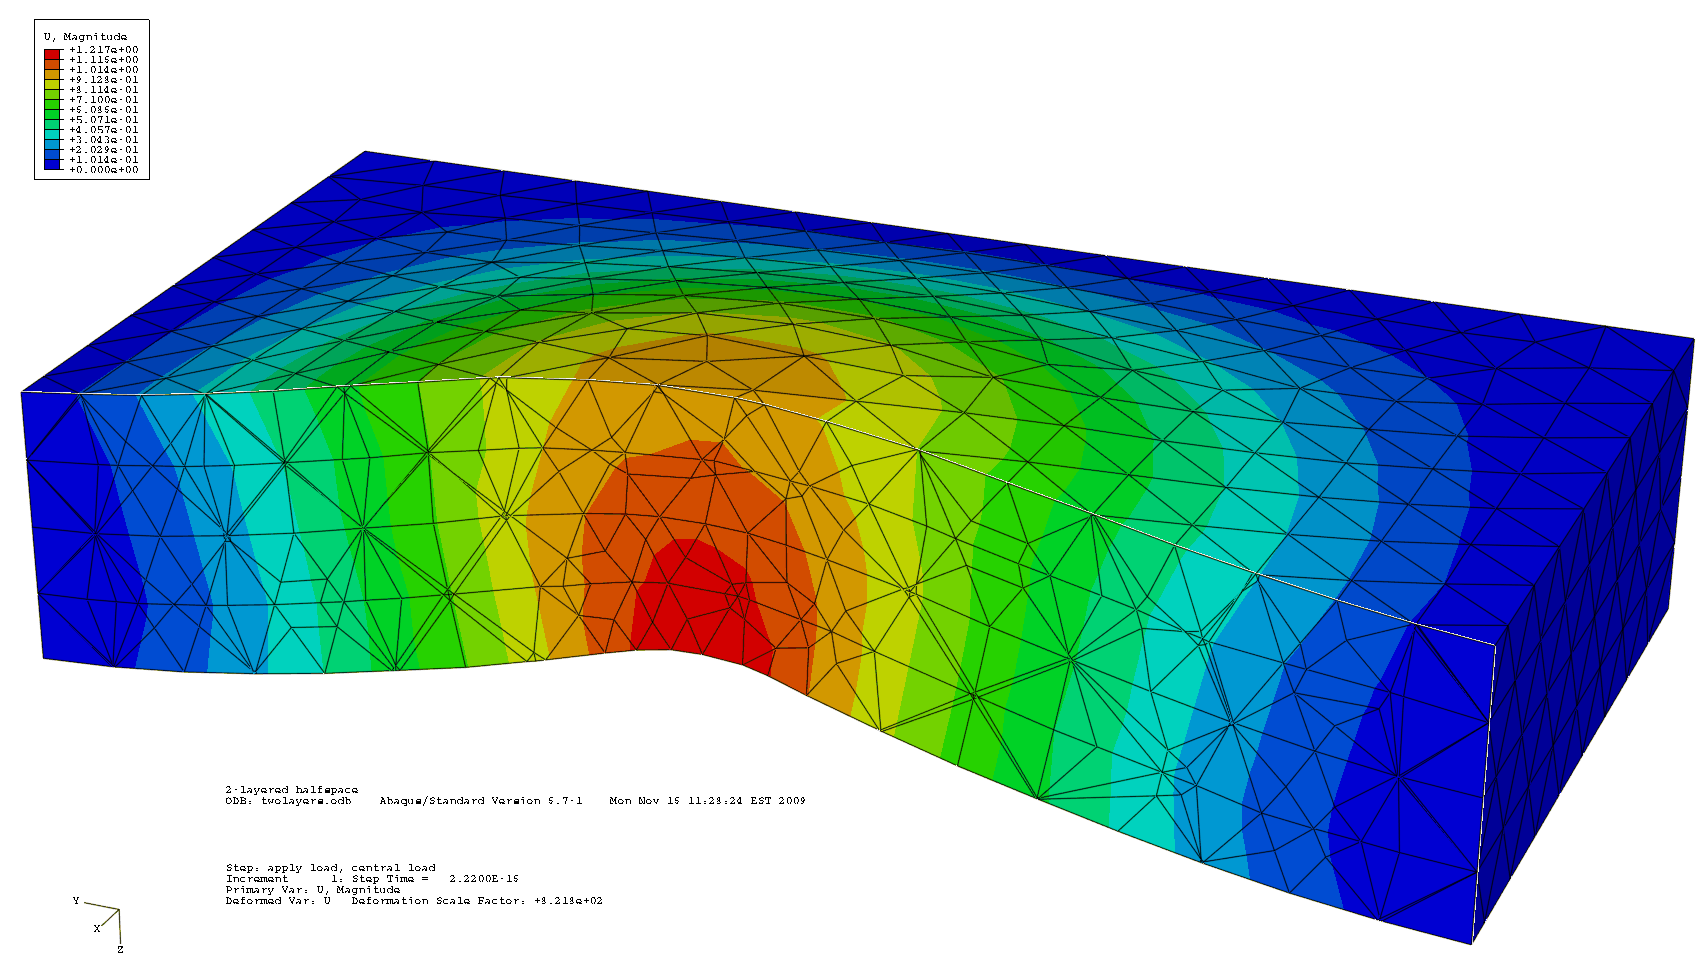
\includegraphics[width=120mm, scale=1]{MeshQualityDeterioration.png}}
  \caption{Example of how elements can be distorted in order to fit a geometry which will result in deterioration of gradient quality (image source: \cite{PoorFEElementShapes})}
\end{figure}


\noindent
Localised metrics associated with the quality of each element have shown to be accurate for predicting the overall quality of a mesh when taking the average for each metric across all elements \cite{DittmerMeshQualityMet}. The quality of an elements shape is important since the stress values which are computed for the area within the element are calculated using the stress values at each of the nodes which enclose it \cite{IntroductionToFE}. Elements are typically deformed near parts of the geometry where its shape simply does not allow a uniform element to be placed, an example of where this has occurred can be seen in figure 2.\\ 

\noindent
Some key shape metrics identified by Dittmer et al include (ideal values are for elements of quadrilateral type as used in  the current prototypes):

\begin{enumerate}[label=\Alph*]
\item Aspect ratio – longest side / shortest side, ideal value is 1
\item Maximum corner angle - widest internal angle to element, ideal is 90\degree
\item Maximum parallel deviation - how skewed the element is, ideal is 0\degree
\end{enumerate}

\section{Description of the work}
\subsection{Aims and Objectives}
The aim of this project is to analyse and design a system for refining a mesh by combining a method from the domain of AI or machine learning with a stress based refinement method. The desirable end result will be a hybrid method of meshing which produces reasonably good solution accuracy whilst requiring less user intervention and reduced computational cost.\\

\noindent
The project can be broken into thee main sections of research and implementation which can each be considered a high level objective:\\ 

\begin{enumerate}[label=\Alph*]

\item The first objective is to research and develop both a traditional stress refinement and an AI re meshing algorithm developed by industry or by academia. These algorithms should be able to run independently on a set of example models.

\item Secondly a process will need to be devised for combining the two re meshing methods to varying degrees will be required. This will make it possible to test the effects of a hybrid method across the same set of models. Through this it can be established whether there is notable benefit to combining the different approaches and if so to what degree is it effective.

\item The third objective will be to use justifiable metrics for assessing the quality of a given mesh. This will allow for a much greater range of hybrid variations to be tried without requiring inspection from an expert. 
\end{enumerate}

\section{System specification}
To demonstrate success in achieving the objectives of the project it is important to have tractability from the requirements through to the solution and lastly verification and validation. This section describes the current systems \textit{functional requirements} (what the system will do) and \textit{non-functional} requirements (its constraints) based upon evaluation of the research I have conducted in conjunction with discussions with the project supervisor: Dr Jason Atkin. Functional requirements have primarily been listed under their respective high level subsystems that are responsible for encapsulating their functionality. \\ 

\noindent
Although it has not been developed as part of the project the application responsible for solving the finite element models has been included as part of the systems requirements since it highly influences the overall scope of the project and much of the design associated with other subsystems which were developed for the project. \\ 

\section{Functional Requirements}

\begin{enumerate}
\item FE integration: System will be able to interface with a third party finite element application

\begin{enumerate}
\item The finite element application’ solver must be able to solve a mesh based on its model configuration.
\item The finite element application’ solver must be able to execute a model programmatically
\item The finite element application’ solver must be able to output stress data at different points on the mesh.
\item The finite element application will provide a graphical representation of the model.
\item It will be possible to manipulate the model that the finite element application uses programmatically.
\item It should be possible to manipulate the model that the finite element application uses from within its graphical user interface.
\end{enumerate}

\item Mesh refinement: System will be able to perform different kinds of finite element mesh refinement

\begin{enumerate}
\item The system will be able to refine a finite element mesh using a stress based refinement method
\item The system will be able to refine a finite element mesh using a non-stress based refinement method

\item A non stress based refinement method will adapt the mesh using background information about mesh design which has been previously trained.

\item The system will be able to combine the two methods to produce a coherent mesh which the FE application is able to successfully solve in order to obtain results for stress and displacement.
\item The system will be able to combine both methods to varying degrees will be performed automatically by the system without direct user intervention.
\item The system will re mesh using both stress and non-stress based refinement using quadrilateral elements.
\item System will adapt weighting associated with each method based upon the metrics computer for the mesh in the systems previous iteration.
\end{enumerate}

\item Quality assessment: System will provide the operator with results about the quality of meshes based on metrics obtained from research.

\begin{enumerate}
\item An assessment will be conducted automatically for every mesh iteration that occurs.
\item System will assess quality based on a variety of metrics to ensure overall robustness of measurement. 
\item The metrics will be computed for both individual elements within the model and for the entire mesh.
\end{enumerate}
\end{enumerate}

\section{Non-Functional Requirements}


\textbf{Design:} The system architecture will be developed using the object oriented design principals of SOLID to allow for clear interfaces between the different functional components. Functional programming practices will be adopted through use of the .NET Language Integrated Query or LINQ framework. This will help to simplify the code and improve reliability. Where functions and classes are written their length will be kept to a minimum to reduce complexity and allow for reuse wherever possible. \\ 

\noindent
\textbf{Documentation:} The system will be comprehensively documented at both a code level and at an architecture level. At a code level C\# doc comments will be written to provide a comprehensive summary of each function. This will allow the tool Doxygen \cite{Doxygen} to generate a full set of developer documentation upon completion of the software implementation which will be included as an appendix. Doc comments will also help to encourage small functions. \\

\noindent
\textbf{General applicability:} In order to demonstrate that hybrid methods are a feasible means of approaching meshing problems the resulting software should be able to successfully execute on a range of models with varying geometry. The range of geometries should be representative of typical structural variation.


\section{System Design}
Since the system is currently a collection of prototypes the final design design is yet to be fully realised. As work on the implementation has progressed however a system architecture that resembles figure 3 below is emerging.

\begin{figure}[!h]
  \centerline{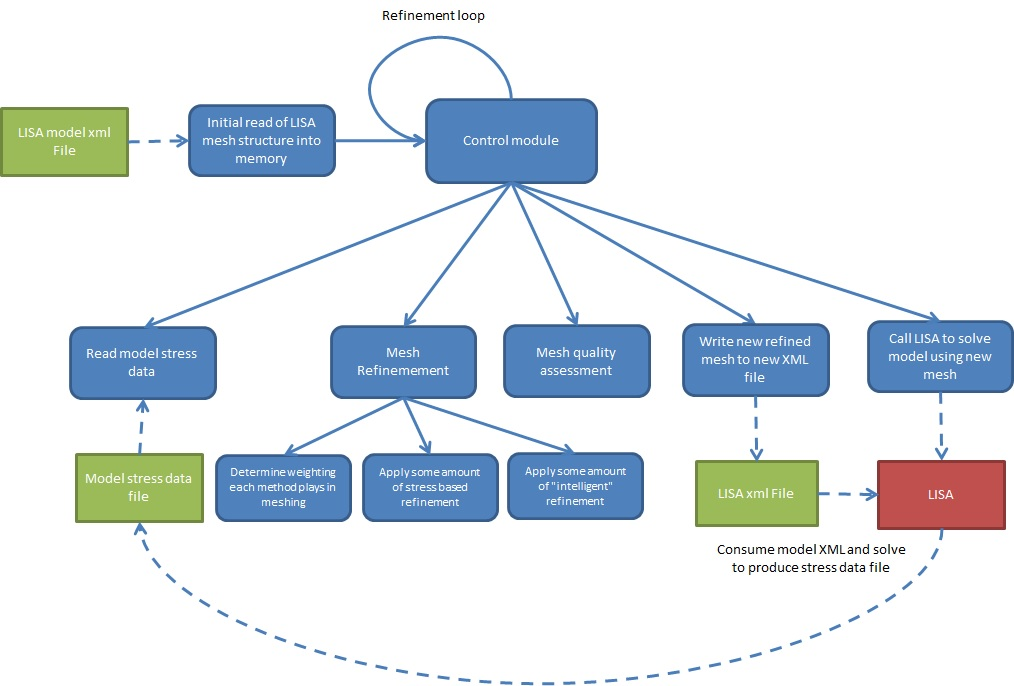
\includegraphics[width=150mm, scale=1]{SystemDesignDiagram.jpeg}}
  \caption{Diagram representing the general structure of the system with interactions between non internal entities such as files and LIA shown using dashed lines}
  \label{fig:h-refinementImp}
\end{figure}


\section{Progress and Current Prototypes}
The following sections describe parts of the project for which implementation work has so far been conducted. These prototype implementations will inform the remainder of the project moving forward.

\subsection{Third Party FE application}

In order to prototype and verify the concept of the hybrid approach it was first important to obtain a finite element solver which could be given a FE model containing data about forces, materials and the mesh structure and then execute the model programmatically so as to obtain stress results. \\ 

\noindent
A multitude of commercial FE tools exist with there being a wide variety in both the complexity and cost associated with each tool. 
Finite element software is typically very expensive due to its high development cost and small customer base. Tools used within industry such as ANSYS typically require a great deal of time in order to become proficient in their usage and can cost in excess of five thousand pounds a year for a single licence \cite{AnsysCost}. It was therefore important to find a tool which was both affordable while also powerful enough to demonstrate a working prototype of the re meshing method.
 
\subsection{LISA}
After reviewing several FE applications used within industry in addition to a variety of less well known ones used within academia and by hobbyists LISA  was selected as the solver application for which to implement  the systems prototypes. \\ 

\noindent
\textbf{Strengths: }LISA as a FE tool allows models of up to 1300 element for free; the full version can be bought for a fee of \$99.99 \cite{LISAWebsite} which is not expensive when compared to other tools on the market. LISA also provides a GUI which allows visual inspection of the model and its mesh; this is particularly useful for observing the output of the meshing algorithms which when observed visually provide a human with a much better understanding of how the method has performed and whether or not there are obvious bugs. \\ 

\noindent
\textbf{Weaknesses: } Due to LISA’s simplicity it does not come with an extensive API allowing for easy programmatic use of its inbuilt features, however it is still possible to interface with LISA through less direct means \cite{LISAManual}. LISA models are stored in .liml files which use XML as a meta mark-up format. The model files contain all the information about the model including the materials used as well as loads and constraints and of course the mesh. It is therefore possible to manipulate a .liml file having parsed its contents before writing a new version of the file which LISA can be called to solve. In order to more easily alter the model it made sense to write a wrapper  for the .liml files to abstract the manipulation of their content.

\subsection{Languages and platforms}
Implementation of re meshing functionality, mesh quality validation and LISA interfaces have so far all been written using C\# with language version 5.0 with Visual Studio 2015 as the development environment on a Windows 10 system. My knowledge and past experience with C\# makes it a suitable language for implementation and will hopefully lead to more rapid development.

\subsection{Prototypes}
Prototypes have so far served as a basis for validating the feasibility of the individual components of the project as well as providing a basis for the full system implementation which will be evolved out of composition of the prototypes. There are three areas that current prototypes have focused these are:

\begin{enumerate}[label=\Alph*]
\item Development of LISA API for easy manipulation of the FE model (as discussed in LISA weaknesses)
\item Implementation of standard re meshing algorithm.
\item Automatic assessment of meshes.
\end{enumerate}

\subsection{LISA API}

Writing the LISA API was the first stage of development for my project. The API was crucial in order to conduct further work on the more advanced prototypes which rely on the existence of different operations in order to easily manipulate the mesh. When a re-meshing iteration occurs the system first reads the .liml file into an equivalent class model, diagrams for which can be seen in figure 4 below. Under each class in this model are the methods and attributes which can be used to adapt the mesh either by the traditional or AI method. Once the mesh model has been adapted it can be assessed by the module responsible for validating the meshes quality and handed back to LISA for further solving.\\
\begin{figure}[!h]
\centering
\begin{subfigure}{.5\textwidth}
  \centering
  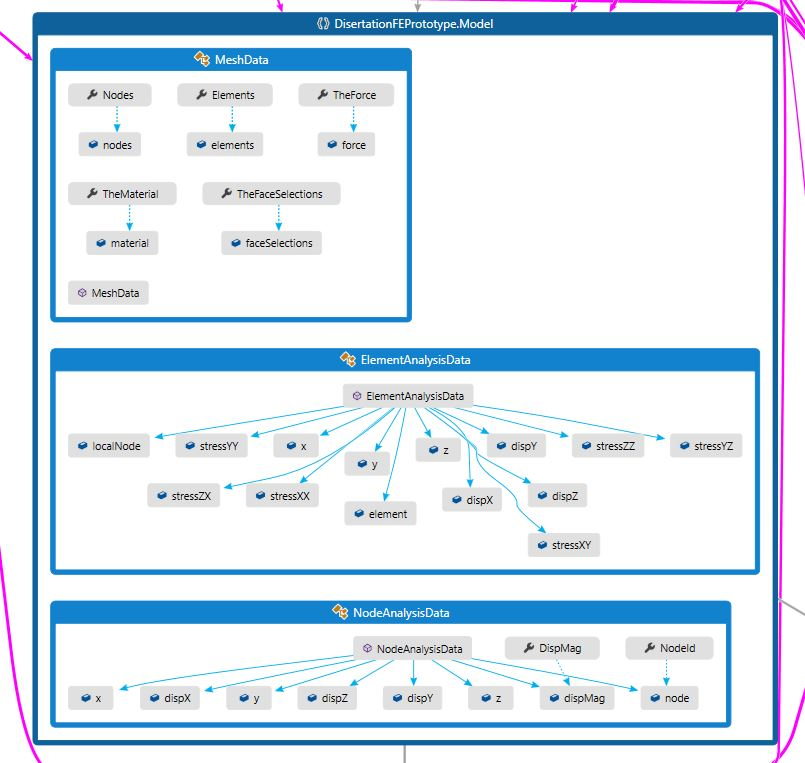
\includegraphics[width=0.9\linewidth]{DissoFEProto-Model.jpg}
  \caption{Model classes}
  \label{fig:sub1}
\end{subfigure}%
\begin{subfigure}{.5\textwidth}
  \centering
  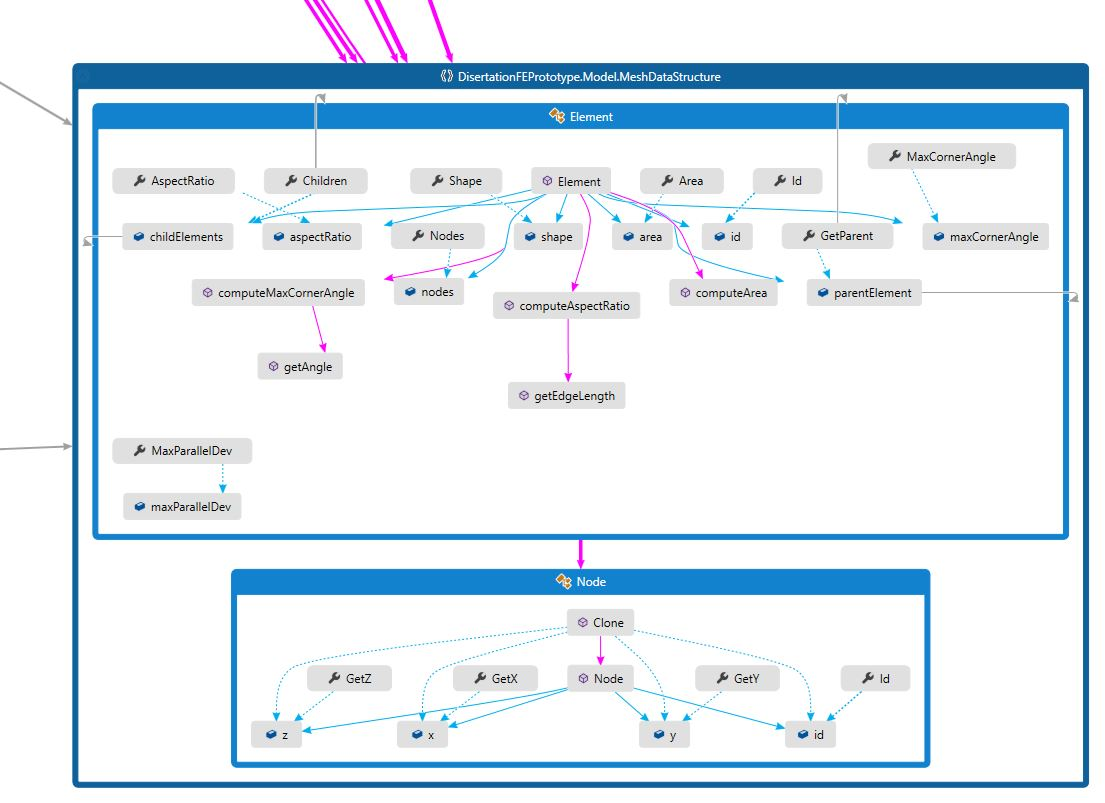
\includegraphics[width=0.9\linewidth]{DissoFEProto-ElemNode.jpg}
  \caption{Element and Node classes}
  \label{fig:sub2}
\end{subfigure}
\label{fig:test}
\end{figure}

\begin{figure}
\centering
\begin{subfigure}{.5\textwidth}
  \centering
  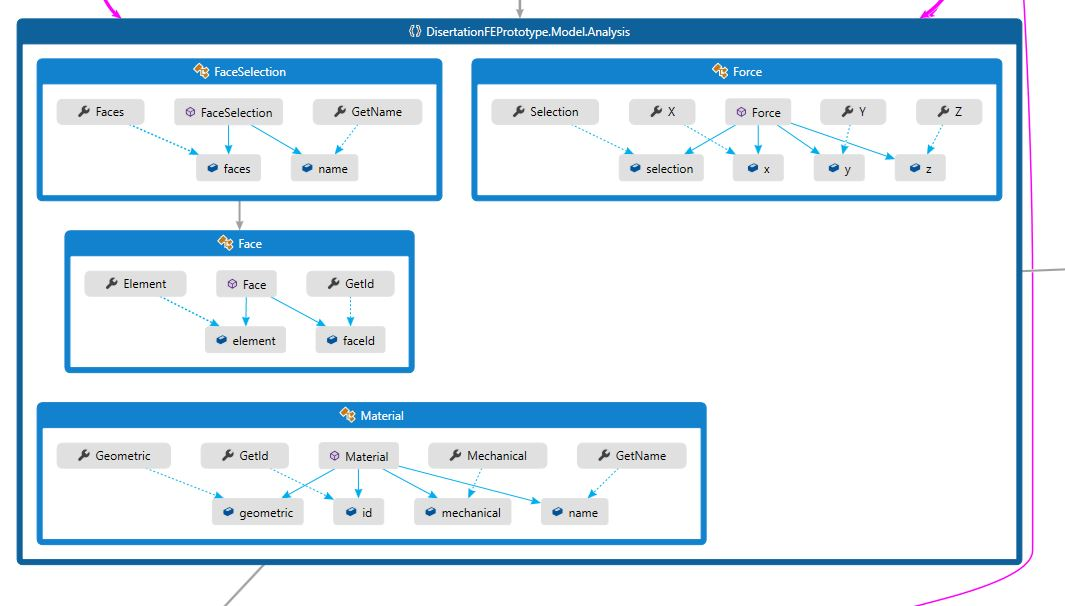
\includegraphics[width=0.9\linewidth]{DissoFEProto-ModelAnalysis.jpg}
  \caption{Model Analysis classes}
  \label{fig:sub1}
\end{subfigure}%
\begin{subfigure}{.5\textwidth}
  \centering
  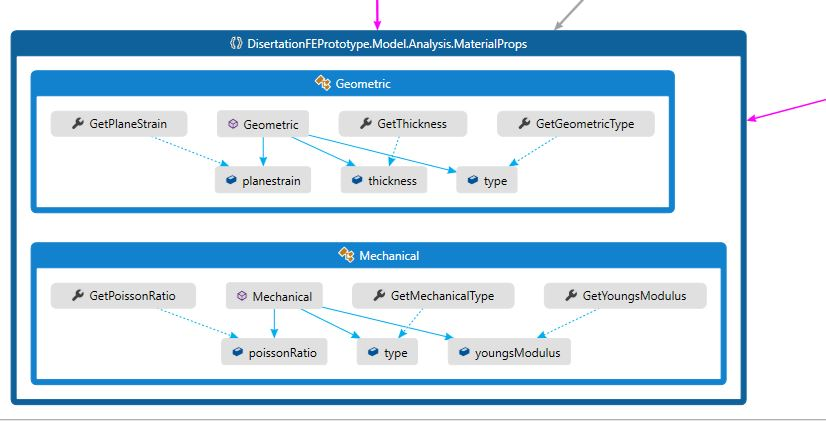
\includegraphics[width=0.9\linewidth]{DissoFEProto-MaterialProps.jpg}
  \caption{Material Property classes}
  \label{fig:sub2}
\end{subfigure}
\label{fig:test}
\caption{Class model to represent .liml file structure used by LISA}
\end{figure}

\newpage
\subsection{Implementation of hierarchical refinement for re meshing}
Having implemented the API to facilitate manipulation of the mesh the next stage was to implement a basic stress based refinement which could be run on a LISA mesh. After reviewing both h-refinement \cite{HandPRefinements} and r-refinement \cite{RRefinement} it was concluded h-refinement would be best to adopt for use in a prototype due to its simplicity and more widespread use \cite{HandPRefinements} despite the fact that the mesh is usually more computationally expensive than it would have been if it was created using r-refinement \cite{RRefinement}\\ 

\begin{figure}[!h]
  \centerline{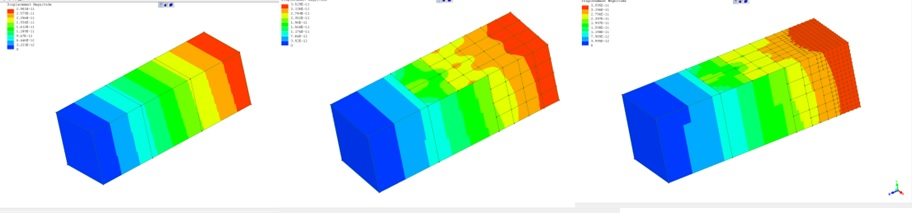
\includegraphics[width=180mm, scale=1]{H-refinementImplementation.jpg}}
  \caption{left to right h-refinement prototype working to expose more detail in stress gradient by applying an increasingly finer mesh. The surface to which the beam is attached runs perpendicularly where the low stress surface coloured dark blue can be seen.}
  \label{fig:h-refinementImp}
\end{figure}

\newpage
\noindent
The prototype implementation of h-refinement which can be seen in figure 5 above has so far been run on a simple cantilever beam problem in LISA. The cantilever beam problem is where a beam attached perpendicular to a solid wall with a force exerted downwards at its end generating sheer stress \cite{cantileverBeam}. The prototype improves the gradient for the problem as follows:

\begin{enumerate}
\item Run initial execution of the model with coarse mesh for basic stress values in each main region.
\item Read in stress and displacement data outputted by LISA.
\item Cross reference LISA stress and displacement data with nodes and elements in the model.
\item If the stress for the element is greater than the average stress of an element within the model then recursively split that element into four smaller elements.
\item Distribute the bending force assigned to parent element across the four sub elements.
\item Repeat steps 2-5 to improve gradient on further runs.
\end{enumerate}


\subsection{Re meshing using Dolsaks ILP knowledge base}
Having successfully implemented an h-refinement method the next key step of the system prototype is to implement the framework for executing the ILP rules published by Dolsak.  So far a fully working prototype of the Dolsak rule based system has not been completed, however implantation of the classes and methods needed to specify the edge relationships as described in Dolsaks papers \cite{DolsakPaper91, DolsakPaper94, appOfILPToFEMeshDesign} \cite{ConsultRuleIntelltSystemFE} is currently under development.

\subsection{Mesh Quality Assessment}
The final area where prototypes have so far been conducted is the development of code for calculating the metrics described by Dittmer that are associated both with individual elements and the entire mesh. For element based metrics there is a need to calculate each metric for each new element that is within the model. Code associated with calculating these values therefore resides within the element class. Due to the fact that each element is initialised with information about the node that comprise it, it is also possible to derive all the geometric characteristics about the individual node that can be used to calculate its various metrics. So far the subsystem for calculating metrics has only been executed on the cantilever beam example described above.


\section{Project Management}

\subsection{Methodology}
Due to the inherently practical nature of the project it is important to combine research of work conducted by the wider academic community with practical prototyping and implementation tasks in order to validate my own hypothesis and demonstrate the feasibility of each project component before proceeding.

\subsection{Time Management}
Management of time for the project will be planned out using the spiral development methodology, where each cycle in the spiral will correspond to either one or two weeks of time on the project. The advantage of adopting the spiral approach is its enforcement of multiple deliverable stages which help reduce risk and ensure that progress is reviewed frequently. The spiral methodology also provides flexibility regarding the order in which tasks take place outside of a cycle iteration, this is necessary when conducing a research project where direction of work is in part dictated by the findings of the research.
A spiral iteration will begin and end with a supervisor meeting. This will allow discussion of progress made during an iteration and serve as a chance to evaluate what are the priorities for the subsequent spiral iteration. 

\subsection{Project Plan}
\noindent
Having discussed each of these stages within supervisor meetings it was possible to extract the following tasks and form a plan to estimate the time scales for each deliverable. A Gantt chart relating planned tasks to their period of undertaking can be seen on page 14.\\ 


\noindent
\textbf{Tasks:}

\begin{enumerate}[label=\Alph*]
\item Write supervisor project Proposal.
\item Review currently available FE tools that I can use as the basis for conducting my work.
\item Conduct research on current applications of AI and machine learning for FEA.
\item Given feasibility of work begin to build basic interfaces with FE tool and consider architecture for tool.
\item Conduct research on mesh assessment metrics allowing for automatic quality check of generated meshes.
- research metrics\\
- investigate building them into prototype of tool
\item Time allocation to catch up with University coursework.
\item Write interim report for dissertation (deadline 08 December).
\item Research possible methods for combining both stress based refinement and AI refinement\\
- explore research methods\\
- implement prototype of composition functions and run iteratively on basic model.
\item Take Christmas time off/revise other modules.
\item Research feasibility of distribution or concurrent execution of problem.
\item Develop/obtain a series of finite element models of increasing complexity to test current prototype on.
\item Having run the developed models look at fixing any problems that may have arisen as a result of increased complexity in geometry.
\item Analyse results from running prototype on range of models and analyse/cross reference results against those reported in papers.
\item Review and update methods before rerunning  them on the models to hopefully achieve improved results.
\item Begin to structure the layout/arguments I want to make for the final dissertation.
\item Write final dissertation (Deadline 6th April 2017).
\end{enumerate}


\section{Personal Reflections}
Comparing the current progress of the project against the plan things are on track to be completed as scheduled. So far I am pleased with both my research efforts and the functionality that I have been able to implement. My primary concern at present is that the ILP generated rules may not perform as well as expected when fully implemented or that they perform well but only for a limited set of geometries, which would be disappointing. While conducting research, development and implementation for the project I have worked methodically to best understand each problem as and when they occur and consider each of the possible solutions before committing to one. I feel this approached has saved me much time and has forced me to reach a better view about what exactly each subsystem should do and how to implement it. In hindsight if I were to repeat the first part of the project again I would have organised my time differently to spend less of it focussed on the details of coursework assignments for other modules into making further progress on the implementation of the rule system.

\newpage
\pagestyle{empty}
\begin{landscape}
\vspace*{1cm}
\hspace*{-3cm}
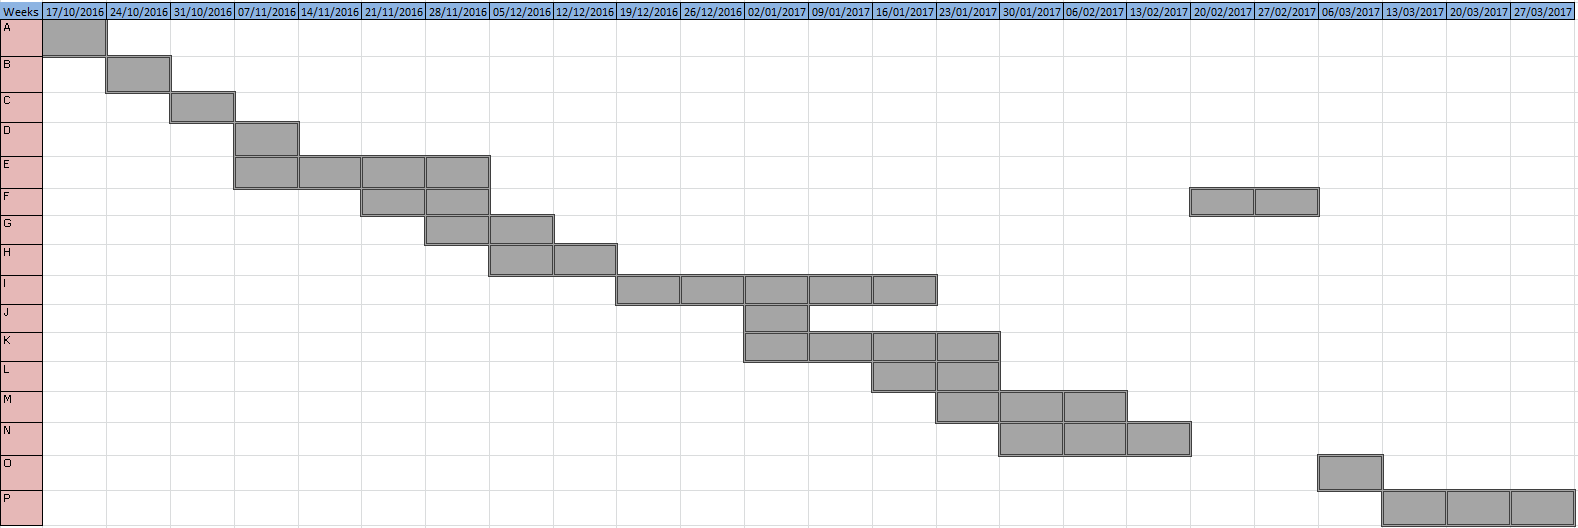
\includegraphics[width =700px, height=300px]{TimePlanUpdated2.png} \par
\hspace*{-1cm}

\end{landscape}

\newpage

\begin{changemargin}{\CMwidth}{\CMheight} 

\addcontentsline{toc}{section}{References}
\begin{thebibliography}{9}

\bibitem{cite0} Max D. Gunzburger, Janet S. Peterson \emph{Finite Element Methods} \url{https://people.sc.fsu.edu/~jburkardt/classes/fem\_2011/chapter1.pdf}

\bibitem{HandPRefinements} Adaptive Finite Element Techniques \url{http://www.cs.rpi.edu/~flaherje/pdf/fea8.pdf}

\bibitem{RRefinement} Scott McRae \emph{r-Refinement grid adaptation algorithms and issues}

\bibitem{DolsakPaper91} Bojan Dolsak and Anton Jezernik \emph{Mesh generation expert system for engineering analysis with FEM}

\bibitem{DolsakPaper94} Bojan Dolsak, Anton Jezernik \emph{A knowledge base for finite element mesh design} Artificial Intelligence in Engineering 9 (1994)

\bibitem{appOfILPToFEMeshDesign} Bojan Dolsak, Stephen Muggleton \emph{The Application of Inductive Logic Programming to Finite Element Mesh Design}

\bibitem{ConsultRuleIntelltSystemFE} Bojan Dolsak, Frank Reig, Reinhard Hackenschmidt \emph{Consultative Rule-Based Intelligent System for Finite Element Type Selection} Research Gate 2016

\bibitem{TraditionalHybridRefinement} Paul Dvorak \emph{Two meshing methods are better than one} \url{http://machinedesign.com/archive/two-meshing-methods-are-better-one}

\bibitem{NeuralNetworks} Larry Manevitz, Malik Yousef, Dan Givoli \emph{Automatic Mesh Generation (for Finite Element Method) Using Self-Organising Neural Networks}

\bibitem{caseBasedReasoning}Abid Ali Khan, Imran Ali Chaudhry2 \& Ali SaroshCase \emph{Case Based Reasoning Support for Adaptive Finite Element Analysis: Mesh Selection for an Integrated System}

\bibitem{MuggletonILP} Stephen Muggleton \emph{Inductive Logic Programming}

\bibitem{Golem} \url{http://www-ai.ijs.si/~ilpnet2/systems/golem.html}

\bibitem{ILPYoutubeLecture}Stephen Muggleton \emph{Logic based and Probabilistic Symbolic Learning} \url{https://www.youtube.com/watch?v=4CwdO5dWW98}

\bibitem{DittmerMeshQualityMet} Jeremy P. Dittmer, C. Greg Jensen, Michael Gottschalk, and Thomas Almy \emph{Mesh Optimisation Using a Genetic Algorithm to Control Mesh Creation Parameters}

\bibitem{PoorFEElementShapes} \url{http://danielpeter.github.io/rays.html}

\bibitem{cite03} Lina Vasiliauskiene, Romualdas BAUŠYS \emph{Intelligent Initial Finite Element Mesh Generation for Solutions of 2D Problems} INFORMATICA, 2002, Vol. 13, No. 2, 239–250 2002

\bibitem{cite04} E.Bellengera,Y.Benhafidb, N.Troussierb \emph{Framework for controlled cost and quality of assumptions in finite element analysis} Finite Elements in Analysis and Design 45 (2009) 25--36

\bibitem{IntroductionToFE} G. P. Nikishkov \emph{INTRODUCTION TO THE FINITE ELEMENT METHOD} \url{http://homepages.cae.wisc.edu/~suresh/ME964Website/M964Notes/Notes/introfem.pdf}

\bibitem{LISAManual} \url{http://www.lisafea.com/pdf/manual.pdf}

\bibitem{cite06}Nam-Ho Kim \emph{STRUCTURAL DESIGN USING FINITE ELEMENTS} http://web.mae.ufl.edu/nkim/eas6939/Opt\_FEM.pdf

\bibitem{cite07}\emph{Type of Finite Elements and Steps in FEA Process}\\
http://highered.mheducation.com/sites/dl/free/0073398144/934758/\\Ch07TypesOfFiniteElementsAndStepsInFEAProcess.pdf 

\bibitem{cantileverBeam} \url{https://www.quora.com/What-is-the-cantilever-beam-What-is-the-advantages-and-disadvantages-of-it}

\bibitem{LISAWebsite} \url{http://www.lisafea.com/purchase.html}

\bibitem{Doxygen} \url{http://www.stack.nl/~dimitri/doxygen/} 

\bibitem{ElementShapeQuality} \url{https://caeai.com/blog/will-poorly-shaped-elements-really-affect-my-solution}

\bibitem{AnsysCost} \url{http://mscnastrannovice.blogspot.co.uk/2013/04/how-much-does-ansys-cost.html}

\bibitem{HighStressCorner} \url{http://www.engineeringanalysisservices.com/moving-mesh-fea-analysis.php}

\end{thebibliography}

\end{changemargin}

\end{document}
